\section{Signal preprocessing}
The vibration signals in a factory environment are inherently full of disturbances. Nearby equipment operation and handling of heavy objects in the surroundings can all contribute to the unwanted chaotic movement in otherwise mostly pure oscillatory motion. In addition, accelerometers suffer from systematic measurement errors in the form of thermal noise, zero-g offset as a result of slight miscalibration, and bias originating from a constant force of gravity. These unavoidable distortions are suppressible to some extent with digital filters. In the preprocessing stage, we consider detrending, noise reduction with adaptive filters, and time synchronous averaging to eliminate interference among components.

\subsection{Detrending}
The oscillatory motion should be centered around the zero level for further manipulation. The constant offset is eliminated simply by subtracting the overall mean from the signal. Moreover high pass DC blocker infinite impulse response (IIR) filter of 1st order can adjust to shifts of the average value over time(Equation~\ref{equ:iir-dc-blocker}). The transition band depends upon the choice of corner frequency $f_{3dB}$ (Fig.~\ref{fig:dc-blocker}).

\begin{equation} \label{equ:iir-dc-blocker}
y_k = (1 - \frac{\omega}{2}) \cdot (x_k  -  x_{k - 1}) + (1 - \omega) \cdot y_{k - 1}; \quad \omega = 2\pi \cdot \frac{f_{3dB}}{f_s}
\end{equation}

A steeper 3~dB attenuation band can be achieved by increasing the order of the filter. Then the cutoff frequency should be such that filter coefficients are fractions to counteract rounding errors~\cite{tittelbach-helmrich_digital_2021}.

\begin{figure}[h]
	\centering
	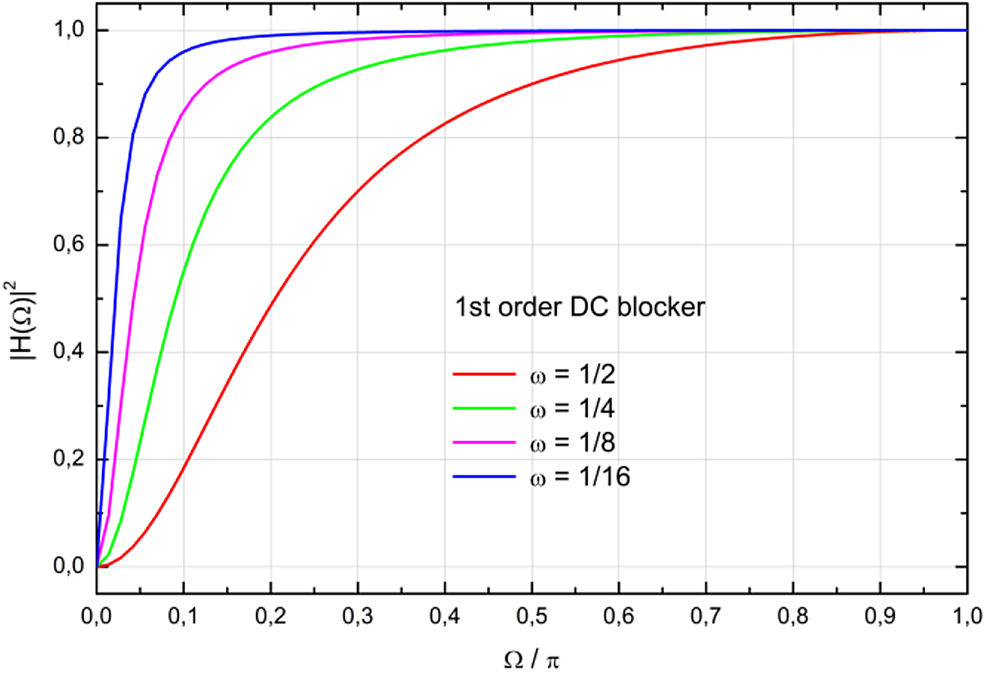
\includegraphics[width=0.7\textwidth]{assets/iir-1-dc-blocker-band.jpg}
	\caption{Transfer function of 1st order DC blocker filters ~\cite{tittelbach-helmrich_digital_2021}}
	\label{fig:dc-blocker}
\end{figure}

The finite impulse response (FIR) filter is not recommended for DC component removal because of the undesirable ripple effect with the small number of taps. Cascaded-integrator-comb (CIC) filters are proposed as an alternative instead~\cite{lyons_understanding_2011}.

\subsection{Adaptive noise cancellation}
Adaptive noise cancellation (ANC) involves an adaptive filter that self-adjusts coefficients through an update algorithm in response to the reference noise signal.  The objective of this filter is to minimize the cost function of mean square error (MSE) in the error signal $e_k$ between signal contaminated with additive Gaussian noise $d_k$ and filter output $y_k$. Additive noise $n_k$ is assumed to be correlated with noise signal $\mathbf{X_k}$~\cite{diniz_adaptive_2020}.

Wiener-Hopf equations solve the optimal gradient of MSE function and provide us with FIR filter coefficient vector $\mathbf{W_k}$.  The least mean squares (LMS) algorithm recursively approximates this analytical solution with the method of steepest descent (Equation~\ref{equ:lms-adaptive-filter})~\cite{diniz_adaptive_2020}. The multiple parameters are to be considered in the evaluation of filter performance: convergence rate, estimated error, and signal-to-noise ratio (SNR).

\begin{ceqn}\begin{align} \label{equ:lms-adaptive-filter}
\mathbf{W}_{k+1} = \mathbf{W}_{k} + 2 \mu \mathbf{X}_{k}  e_k
\end{align}\end{ceqn}

The convergence stability is affected by step size $\mu$ which is bounded from above with the inverse of the maximal eigenvalue of input covariance matrix $\lambda_{max}$. The normalized least mean squares (NLMS) can handle input of varying scales  (Equation~\ref{equ:nlms-adaptive-filter}).

\begin{ceqn}\begin{align} \label{equ:nlms-adaptive-filter}
\mathbf{W}_{k+1} = \mathbf{W}_{k} + \frac{\mu}{\lVert\mathbf{X}_{k}\rVert^2} \mathbf{X}_{k}  e_k
\end{align}\end{ceqn}

\begin{figure}[h]
	\centering
	
\includegraphics[width=0.8\textwidth]{assets/adaptive-filter.png}
	\caption{Adaptive noise cancellation filter diagram}
	\label{fig:adaptive-filter}
\end{figure}
\bigbreak

\subsection{Time synchronous averaging}
Time synchronous averaging (TSA) diminishes the impact of vibration sources unrelated to the rotational frequency and its harmonics. TSA averages time-domain waveform over $N$ points and aligns it to a synchronization pulse with period $T$ (Equation~ref{equ:tsa-average}). This technique has been successfully applied to the gearbox and bearing fault diagnosis~\cite{davies_handbook_2012,nandi_condition_2019}
\begin{ceqn}\begin{align}
x_{TSA} = \frac{1}{N} \sum_{n = 0}^{N - 1}{x(t + nT)}
\label{equ:tsa-average}
\end{align}\end{ceqn}


\section{Feature engineering}
Raw numerical vectors after preprocessing are merely low-level descriptors of the underlying physical phenomena. At first, these incomprehensible sequences of numbers are reduced to summary attributes called features in the process of feature discovery. Normalization and linear transformations are applied here to discriminate different categories in the feature space. The most informative set of features is obtained with feature selection methods for the diagnostic model. Features can be hand-crafted. Likewise, they can be learned implicitly within the model representation or explicitly as an optimization problem solution.  

\subsection{Feature extraction}
Predictive maintenance has ideal prerequisites for the application of feature engineering because the signal is usually pseudo-stationary, and the trend monitoring variables come out of extensive domain expertise in mechanics. The advantages of add-in extraction effort, as opposed to processing samples unmodified, are to gain better classification precision and reduce computational burden and storage capacity downstream with dimensionality reduction techniques~\cite{johnson_feature_2019}. It is important to note that the design of features is not a standalone step in the machine learning pipeline but it should be performed iteratively to improve the target model.  Signal features are computed in the time domain, frequency domain, and time-frequency domain~\cite{brito_fault_2021}. 

\subsubsection{Time domain features}
The most widely found features in the literature are rudimentary statistical measures of the central moment: mean, variance, standard deviation, skewness, and kurtosis~(Tab.~\ref{tab:td-features}). Statistics can be calculated in any domain, but the mean value is not to be used in detrended data. The vibration severity metrics out of technical standards are also highly regarded. The characteristics of amplitude include root mean square, peak-to-peak, and maximum. \cite{mostafavi_novel_2021}.

The other significant time-domain attributes are derived as ratios of previous simpler ones. These ratios are crest factor, margin factor, impulse factor, and shape factor~(Tab.~\ref{tab:td-features})~\cite{nandi_condition_2019}. Many articles have been successful in bearing fault detection out of transients in impulsive signals with kurtosis, crest factor, and margin indicators \cite{brito_fault_2021}. It is also suggested that the shape factor can signify unbalance and misalignment faults~\cite{nandi_condition_2019}.

\begin{table}[h]
\renewcommand{\arraystretch}{1.5}
\begin{adjustbox}{width=\columnwidth,center}
\begin{tabular}{|l|l|l|l|}
\hline
\textbf{Feature}            & \textbf{Equation}                                                                    & \textbf{Feature}        & \textbf{Equation}                                                                                                  \\ \hline
\textit{Standard deviation} & $ \sigma = \sqrt{\frac{1}{N}\sum_{i = 1}^{N}{\left(x_i - \bar{x}\right)^2}} $        & \textit{Crest factor}   & $ X_{cf} = \frac{max(|x_i|)}{\left( \frac{1}{N} \sum_{i=1}^{N}{x_i^2} \right)^\frac{1}{2}} $                       \\ \hline
\textit{Skewness}           & $ X_{sv} = \frac{1}{N}\sum_{i = 1}^{N}{\left(\frac{x_i - \bar{x}}{\sigma}\right)^3}$ & \textit{Margin factor}  & $ X_{mf} = \frac{max(|x_i|)}{\left( \frac{1}{N} \sum_{i=1}^{N}{\sqrt{|x_i|}} \right)^2} $                          \\ \hline
\textit{Kurtosis}           & $ X_{kv} = \frac{1}{N}\sum_{i = 1}^{N}{\left(\frac{x_i - \bar{x}}{\sigma}\right)^4}$ & \textit{Impulse factor} & $ X_{if} = \frac{max(|x_i|)}{\frac{1}{N} \sum_{i=1}^{N}{|x_i|}} $                                                  \\ \hline
\textit{Root mean square}   & $ X_{rms} = \left(\frac{1}{N}\sum_{i = 1}^{N}{x_i^2}\right)^\frac{1}{2}$             & \textit{Shape factor}   & $ X_{sf} = \frac{\left( \frac{1}{N} \sum_{i=1}^{N}{x_i^2} \right)^\frac{1}{2}}{\frac{1}{N} \sum_{i=1}^{N}{|x_i|}}$ \\ \hline
\textit{Peak-to-peak}       & $ X_{ppv} = \max(x_i) - \min(x_i) $                                                  & \textit{Maximum}        & $ X_{max} = \max(|x_i|) $                                                                                          \\ \hline
\end{tabular}
\end{adjustbox}
\caption{Time domain features}
\label{tab:td-features}
\end{table}

\subsubsection{Frequency domain features}
The mechanical faults present themselves as oscillatory patterns which are combinations of frequencies with various amplitudes. The Fourier transform is one of the prominent strategies in power spectral density estimation. Experts on vibrodiagnostics utilize it as a primary signal processing technique for data analysis as it is recommended in ISO 13373 standard. 

The inherent symmetries in the Fourier matrix made it possible to invent an efficient implementation of the Fast Fourier transform (FFT) algorithm with time complexity $O(n \log n)$. The drawback of the plain spectral analysis is the lack of resolution in events that occurred at distant time instants, and so their spectral components might adversely blend in together. 

In the frequency domain, we can obtain spectral centroid, spectral kurtosis, spectral roll-off, spectral flux, energy in frequency bands, and energy ratio \cite{peeters_large_2004}. In geometry terms, the spectral centroid represents the barycenter of the frequency magnitude plot. Spectral roll-off gives a notion about the spectral distribution because it finds the frequency $f_c$ below which 95\% of the signal energy is contained. The energy in the roll-off calculation is summed up to the Nyquist limit: $f_s / 2$.  Spectral flux is according to the definition normalized cross-correlation between two successive amplitude spectra. The result of one means the spectra are the most dissimilar.

The frequencies related by integer ratio known as harmonics may originate from higher order oscillation modes of the same shaft or other elastic rod supported on both ends. Several harmonics features have been proposed. Ones worth investigating are fundamental frequencies, noisiness, inharmonicity, and harmonic spectral deviation. Noisiness as a harmonic feature is a ratio of noise (non-harmonic components) energy to the total contained energy. Inharmonicity measures the divergence of spectral components from a purely harmonic signal with a value of 0. The inharmonic spectrum has an inharmonicity value of 1. Harmonic spectral deviation adds up differences of harmonic peaks from the spectral envelope \cite{peeters_large_2004}. 

If a single principal frequency exists, it can be determined with maximum likelihood estimation. Such frequency would explain the signal spectrum the best \cite{peeters_large_2004}.  The frequency spectrum is a discrete set of amplitudes where peaks have to be reliably identified to create representative attributes.
The essential peak-finding approaches are based either on magnitude or gradient. All found extrema are commonly filtered with the magnitude of prominences and the widths at half prominence.  In the magnitude-based method, middle point $x_i$ is compared to neighboring two points and the peak is then: $x_{i−1} < x_i > x{i+1}$. The gradient-based method evaluates the first derivative at the point which is equal to zero in case the point is local maximum, local minimum, or inflection point \cite{adikaram_non-parametric_2016}.

A substantial improvement is a robust non-parametric peak identification named \emph{MMS} based on the sum of terms in an arithmetic progression based on maximum, minimum, and sum. MMS max-min finder in the elementary form processes points in the window of length 3, it advances one point and deems its middle point as a local extremum if it satisfies equalities below. Equation~\ref{equ:mms-maxima} is for the peak and Equation~\ref{equ:mms-minima} is for the valley. The filtration techniques are incorporated in the adaptations of MMS algorithm: MMS-WBF, MMS-SG, MMS-LH~\cite{adikaram_non-parametric_2016}.

\begin{ceqn}\begin{align}
\mathrm{MMS}_{\mathrm{max}} = \mathrm{MMS}_{\mathrm{max|mid}} \\
\frac{a_{max} - a_{min}}{S_3 - a_{min} \cdot 3} = \frac{a_{mid} - a_{min}}{S_3 - a_{min} \cdot 3}
\label{equ:mms-maxima}
 \end{align}\end{ceqn}

\begin{ceqn}\begin{align}
\mathrm{MMS}_{\mathrm{min}} = \mathrm{MMS}_{\mathrm{min|mid}} \\
\frac{a_{max} - a_{min}}{a_{max} \cdot 3 - S_3} = \frac{a_{max} - a_{mid}}{a_{max} \cdot 3 - S_3}
\label{equ:mms-minima}
 \end{align}\end{ceqn}

Multiple harmonic series and the sidebands can be separated into a discrete set of frequency components, each with central frequency, uncertainty, and amplitude $C_i(v_i, \delta v_i, A_i)$ by an exhaustive search algorithm. Harmonic family identification is a non-trivial problem because of the spectrum estimation errors. The criterium is proposed to select harmonic at the minimal distance from the true fundamental frequency multiple~(Equation~\ref{equ:harmonic-search}). Two series with the same fundamental frequency are merged and thought of as a modulation series \cite{gerber_identification_2013}.

\begin{ceqn}\begin{align}
v_i^{(r)} = \frac{v_j}{\min{|v_j - r \cdot v_i|}}
\label{equ:harmonic-search}
\end{align}\end{ceqn}
 
\begin{table}[h]
\renewcommand{\arraystretch}{1.5}
\begin{adjustbox}{width=\columnwidth,center}
\begin{tabular}{|l|l|l|l|}
\hline
\textbf{Feature}           & \textbf{Equation}                                                                                                 & \textbf{Feature}                     & \textbf{Equation}                                                                               \\ \hline
\textit{Spectral centroid} & $ X_{fc} = \frac{\sum_{i = 0}^{N - 1}{f_i \cdot s(f_i)}}{\sum_{i = 0}^{N - 1}{s(f_i)}}$                           & \textit{Noisiness}                   & $X_{noisi} = \frac{\sum_{k \notin h}^{N}E_k}{\sum_{i = 1}^{N}E_i} $                             \\ \hline
\textit{Spectral roll-off} & $ \sum_{0}^{f_c}a^2(f) = 0.95 \sum_{0}^{f_s / 2}a^2(f)$                                                           & \textit{Inharmonicity}               & $X_{inharmo} = \frac{2}{f_0} \cdot \frac{\sum_h | f(h) - h \cdot f_0| * a^2(h)}{\sum_h a^2(h)}$ \\ \hline
\textit{Spectral flux}     & $X_{\mathrm{flux}} = 1 - \frac{\sum_k a(t-1, k) \cdot a(t,k)}{\sqrt{\sum_k a(t-1, k)^2} \sqrt{\sum_k a(t, k)^2}}$ & \textit{Harmonic spectral deviation} & $ X_{\mathrm{HDEV}} = \frac{1}{H}\sum_h(a(h) - SE(h))$                                          \\ \hline
\textit{Energy}            & $ E_s = \sum_{i = 0}^{N - 1}|x(t)|^2 $                                                                            & \textit{Energy ratio}                & $E_i = \frac{E_i}{\sum_{i = 1}^{N}E_i} $                                                        \\ \hline
\end{tabular}
\end{adjustbox}
\caption{Frequency domain features}
\label{tab:td-features}
\end{table}

%TODO
\subsubsection{Time-Frequency domain features}
% Time frequency + WPT (Energy, entropy) - gain resolution in time domain, CWT,WPT, discussed in detail later.
The short-time Fourier transform (STFT) splits the time-domain signal at the equal length intervals and combines these chunks with window function to eliviate spectral leakage as a loss of resolution.
\cite{zhuo_research_2022}
\cite{mostafavi_novel_2021}




% Feature Engineering for Machine Learning
\cite{zheng_feature_2018}
% Feature Engineering and Selection: A Practical Approach for Predictive Models
\cite{johnson_feature_2019}

% A Novel Online Machine Learning Approach for Real-Time Condition Monitoring of Rotating Machines
% - list of features
\cite{mostafavi_novel_2021}

% A New Statistical Features Based Approach for Bearing Fault Diagnosis Using Vibration Signals
% - knn with manhalobis distance
% - select features manually as oposed to CNN and RNN
\cite{altaf_new_2022}


% Fault Detection of Bearing: An Unsupervised Machine Learning Approach Exploiting Feature Extraction and Dimensionality Reduction
\cite{brito_fault_2021}

% FFT - Short Time Fourier Transform with Hamming window and Welch averaging



% A large setof audio features for sound description
\cite{peeters_large_2004}
% Research on online intelligent monitoring system of band saw blade wear status based on multi‑feature fusion of acoustic emission signals
\cite{zhuo_research_2022}
% Early Detection of Imbalance in Load and Machine In Front Load Washing Machines by Monitoring Drum Movement
\cite{mohammadi_early_2020}
% A Data Mining based Approach for Electric Motor Anomaly Detection Applied on Vibration Data
\cite{egaji_data_2020}
% Condition Monitoring with Vibration Signals
\cite{nandi_condition_2019}
% Vibration Analysis for IoT Enabled Predictive Maintenance
\cite{jung_vibration_2017}

\paragraph{Statistical measures}
\begin{itemize}
\item Energy
\item Spectral negentropy
	% Spectral negentropy and kurtogram performance comparison for bearing fault diagnosis
	\cite{avoci_spectral_2020}
\item TKEO - Teager-Kaiser energy operator
	%Application of Teager–Kaiser Energy Operator in the Early Fault Diagnosis of Rolling Bearings
	\cite{shi_application_2022}
\end{itemize}

\paragraph{Wavelet signal decompositions}

\begin{itemize}
\item CWT-SST - Synchrosqueezing Wavelet Transform
	% The fast continuous wavelet transformation (fCWT) for real-time, high-quality, noise-resistant time–frequency analysis
	\cite{arts_fast_2022}
	% A Concentrated Time–Frequency Analysis Tool for Bearing Fault Diagnosis
	\cite{yu_concentrated_2020}
	% Applications of the synchrosqueezing transform in seismic time-frequency analysis
	\cite{herrera_applications_2014}

\item WPD - Wavelet Packet Decomposition  - to approximation and detail coef. (Fejer-Korovkin wavelet)
	% Wavelet Packet Feature Extraction for Vibration Monitoring
	\cite{yen_wavelet_2000}
	% A wavelet approach to dimension reduction and classification of hyperspectral data
	\cite{wickmann_wavelet_2007}
	% The MFBD: a novel weak features extraction method for rotating machinery
	\cite{song_mfbd_2021}

\item EWT - Empirical Wavelet Transform - (Meyer wavelet)
	% Empirical Wavelet Transform - Gilles
	% On the computational complexity of the empirical mode decomposition algorithm
	\cite{wang_computational_2014}
	% Novel self-adaptive vibration signal analysis: Concealed component decomposition and its application in bearing fault diagnosis
	\cite{tiwari_novel_2021}
	% The MFBD: a novel weak features extraction method for rotating machinery
	\cite{song_mfbd_2021}
	% Fault Feature Extraction and Enhancement of Rolling Element Bearings Based on Maximum Correlated Kurtosis Deconvolution and Improved Empirical Wavelet Transform
	\cite{li_fault_2019}
	% An Improved Empirical Wavelet Transform for Noisy and Non-Stationary Signal Processing
	\cite{zhuang_improved_2020}
	% Time and frequency domain scanning fault diagnosis method based on spectral negentropy and its application
	\cite{yonggang_time_2020}
	% An Adaptive Spectrum Segmentation Method to Optimize Empirical Wavelet Transform for Rolling Bearings Fault Diagnosis
	\cite{xu_adaptive_2019}
	% Improved empirical wavelet transform (EWT) and its application in non‑stationary vibration signal of transformer
	\cite{ni_improved_2022}
\end{itemize}


\subsection{Feature transformation}
\cite{zheng_feature_2018}

\subsubsection{Normalization}
 (min-max, standardize)


\subsubsection{Box-Cox transform}

to normal distribution
\begin{ceqn}\begin{align}
\widetilde{x} =
\begin{cases}
\frac{x^\lambda - 1}{\lambda} \quad \mathrm{if} \;\lambda \neq 0, \\\\ 
ln(x)\quad \mathrm{if}\;\lambda = 0
\end{cases}
\label{equ:box-cox-transform}
\end{align}\end{ceqn}

\subsubsection{Principal Component Analysis}
%  (PCA)
% \cite{brito_fault_2021}

\subsection{Feature selection}
% Add citations to usage of different features
Subset generation % p.193
Subset evaluation
Stopping criteria
Validation

\cite{nandi_condition_2019} % p.192
Filter method - SelectKBest  in evaluation phase
\begin{itemize}
\item Variance Threshold
\item Pearson correlation
\item ANOVA F-value
\item Mutal information
\item Fisher score
\item Spectral feature selection algorithm (SPEC)
\end{itemize}
